\documentclass[10pt, a4paper]{report}
\special{papersize=210mm, 297mm}
\usepackage[english]{babel}
\usepackage[utf8x]{inputenc}
\usepackage[left=2.5cm, right=2.5cm, top=2.5cm]{geometry}
\renewcommand{\baselinestretch}{1.4}
\usepackage[toc,page]{appendix}
\pagenumbering{alph}

\usepackage{amsmath}
\usepackage{graphicx}
\usepackage{float}
\graphicspath{{images/} {diagrams/}}

%\usepackage{showframe}
\usepackage{fullpage}

\usepackage{url}
%\usepackage{natbib} % for author-date citation \citep{}, \citet[]
%\usepackage{hyperref}
%\usepackage[nottoc]{tocbibind}
\usepackage{listings}
\usepackage{verbatim}
\usepackage{color}

\definecolor{dkgreen}{rgb}{0,0.6,0}
\definecolor{gray}{rgb}{0.5,0.5,0.5}
\definecolor{mauve}{rgb}{0.58,0,0.82}

\lstset{frame=tb,
	language=java,
	aboveskip=5mm, belowskip=3mm, showstringspaces=false,
	columns=flexible, basicstyle={\small\ttfamily},
	numbers=none, numberstyle=\tiny\color{gray},
	keywordstyle=\color{blue},
	commentstyle=\color{dkgreen},
	stringstyle=\color{mauve},
	breaklines=true,
	breakatwhitespace=true,
	tabsize=3
}


\usepackage{multirow}
\usepackage{array}
\newcolumntype{L}[1]{> {\raggedright\let\newline\\\arraybackslash\hspace{0pt}}m{#1}}
\newcolumntype{C}[1]{>{\centering\let\newline\\\arraybackslash\hspace{0pt}}m{#1}}
\newcolumntype{R}[1]{>{\raggedleft\let\newline\\\arraybackslash\hspace{0pt}}m{#1}}

\pagenumbering{arabic}

\begin{document}
	
	%======================================================================
	
	\begin{titlepage}
		
		\newcommand{\HRule}{\rule{\linewidth}{0.5mm}}
		
		\center
		
		\vspace{-20pt}
		
\includegraphics[width=100pt]{../images/FMI-03.png}\\[1.0cm]
		
		\textsc{\LARGE West University of  Timisoara}\\[0.5cm]
		\textsc{\Large Faculty of Mathematics and Computer Science}\\[0.5cm]
		\textsc{\large Study Program: \\Computer Science in English}\\[3cm]
		\textsc{\Huge Master Dissertation}\\[5cm]
		
		\begin{minipage}{0.4\textwidth}
			\begin{flushleft} \large
				\textbf{COORDINATOR:}\\
				Associate Prof. Marc Eduard \textsc{Frîncu}
			\end{flushleft}
		\end{minipage}
		~
		\begin{minipage}{0.4\textwidth}
			\begin{flushright} \large
				\textbf{GRADUATE:} \\
				Maria Minerva \textsc{Vonica}
			\end{flushright}
		\end{minipage}\\[0.5cm]
			
		\vfill
		{\large Timi\c{s}oara \\2021}\\
		\vfill
		
	\end{titlepage}
	
	% =====================================================================
	
	\begin{titlepage}
		
		\newcommand{\HRule}{\rule{\linewidth}{0.5mm}}
		
		\center
		
		\textsc{}\\[.7cm]
		
		\textsc{\LARGE West University of  Timi\c{s}oara}\\[0.5cm]
		\textsc{\Large Faculty of Mathematics and Computer Science}\\[0.5cm]
		\textsc{\large Study Program: \\Computer Science in English}\\[4.5cm]
		
		\textsc{\Huge Master Dissertation}\\[2cm]
		
		{\Huge \bfseries Name}\\[6cm]
		
		\begin{minipage}{0.4\textwidth}
			\begin{flushleft} \large
				\textbf{COORDINATOR:}\\
				Associate Prof. Marc Eduard \textsc{Frîncu}
			\end{flushleft}
		\end{minipage}
		~
		\begin{minipage}{0.4\textwidth}
			\begin{flushright} \large
				\textbf{GRADUATE:} \\
				Maria-Minerva \textsc{Vonica}
			\end{flushright}
		\end{minipage}\\[0.5cm]
		\vfill
		{\large Timi\c{s}oara\\ 2021}\\
		
		\vfill
		
	\end{titlepage}

	% =====================================================================
	
	\chapter{Application}
	\section{Dataset}
	In order to build the dataset, we made use of the freely available data from the Landsat Archive, specifically from collection 1, level 1. This consists of data products generated from Landsat 8 Operational Land Imager/Thermal Infrared Sensor, Landsat 7 Enhanced Thematic Mapper Plus, Landsat 4-5 Thematic Mapper, and Landsat 1-5 Multispectral Scanner instruments \cite{C1L1}. For the purpose of this paper, we will focus only on images collected from the Landsat 8 satellite.
	
	\subsection{World Glacier Inventory}
	The World Glacier Inventory (WGI) proves to be a useful resource for building our dataset, since it contains information for over 130,000 glaciers. Inventory parameters include geographic location, area, length, orientation, elevation, and classification. The WGI is based primarily on aerial photographs and maps with most glaciers having one data entry only. Hence, the data set can be viewed as a snapshot of the glacier distribution in the second half of the 20th century. It is based on the original WGI (WGMS 1989) from the World Glacier Monitoring Service \cite{WGI}.  
	
	There are a number of ways to retrieve data from the inventory:
	\begin{itemize}
		\item download the entire database in a single ASCII text file (wgi\_feb2012.csv);
		\item search by parameter using the Search Inventory interface;
		\item extract regions through the Extract Selected Regions interface.
	\end{itemize}

	The ASCII text file will be used with the purpose to define which are the glaciers to be included in the dataset to be built. An example of how this file looks like can be found in Figure 1.1.
	
	\begin{figure}[h]
		\centering
		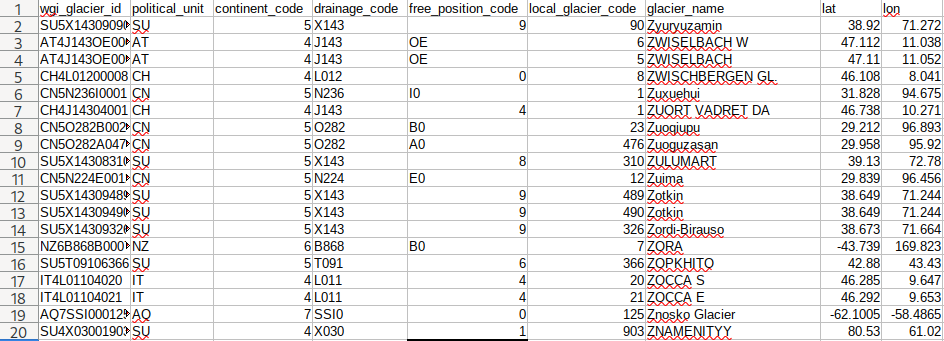
\includegraphics[scale=0.5]{../images/wgi_ASCII_file.png}
		\caption{WGI ASCII}
		\label{fig:WGI_ASCII}
	\end{figure}
	
	The \emph{parameters} which will be extracted for the dataset construction are the following:
	\begin{itemize}
		\item \textit{wgi\_glacier\_id}: unique id representing one glacier (or part of it, if the coverage area is larger);
		\item \textit{glacier\_name}: name of the glacier (if it has one);
		\item \textit{lat}: latitude of the glacier;
		\item \textit{lon}: longitude of the glacier.
	\end{itemize}

	\subsection{Download}
	
	Through the ASCII WGI text file we can pick which glacier we want to download based on its coordinates, by implementing an endpoint of the the SpatioTemporal Asset Catalog API: \url{http://nsidc.org/data/glacier_inventory/index.html} \cite{STAC}. We will also specify the maximum allowed cloud coverage and the bounding box for the searched area, which is calculated based on the latitude and longitude values extracted from the ASCII WGI text file.

	\chapter{Implementation}
	\section{Download}
	
	
	\tableofcontents{}
	\addcontentsline{toc}{chapter}{List Of Figures}
	\listoffigures{}
	\addcontentsline{toc}{chapter}{List Of Tables}
	\listoftables{}
	
	\bibliographystyle{alpha}
	\bibliography{references}
		
	\chapter{Glossary}
	
	% ==================================================================
	
	\section{Acronyms}
	
		\begin{table} [H]
		\centering
		\begin{tabular} {|  l | L{10cm} |}
			\hline
			WGI & World Glacier Inventory \\ [0.2ex]
			\hline
		\end{tabular}
		\caption{Acronyms table }
		\label{table:acron}
	\end{table}
	\end{document}
